\documentclass[tikz]{standalone}

\usetikzlibrary{positioning, calc, decorations.pathreplacing}

\begin{document}
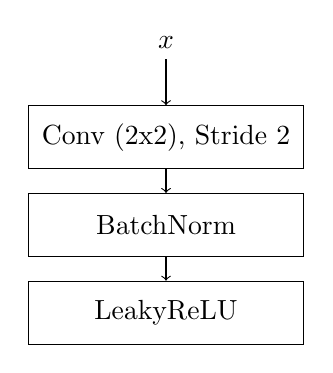
\begin{tikzpicture}

  \node[draw=black, minimum width=3.5cm, minimum height=0.8cm] (conv) {Conv (2x2), Stride 2};
  \node[draw=black, minimum width=3.5cm, minimum height=0.8cm, below=0.3cm of conv] (bn) {BatchNorm};
  \node[draw=black, minimum width=3.5cm, minimum height=0.8cm, below=0.3cm of bn] (lr) {LeakyReLU};

  \draw[<-] (conv) -- ++(0,1) node[above, pos=1] {$x$};
  \draw[->] (conv) -- (bn);
  \draw[->] (bn) -- (lr);
\end{tikzpicture}
\end{document}
